% IEEE Journal Paper Template
% Federated Continual Learning via Dual-Teacher Knowledge Distillation
% Reproducibility study: FedAvg vs FLwF-2 across MNIST / FMNIST / CIFAR-10
% with IID and Dirichlet non-IID partitions across 10/50/100 clients.
% Implementation: Flower (flwr) + PyTorch.

\documentclass[journal]{IEEEtran}

\usepackage{cite}
\usepackage{amsmath,amssymb,amsfonts}
\usepackage{algorithmic}
\usepackage{algorithm}
\usepackage{graphicx}
\usepackage{textcomp}
\usepackage{xcolor}
\usepackage{booktabs}
\usepackage{multirow}
\usepackage{array}
\usepackage{url}
\usepackage{hyperref}
\usepackage{pifont}

\graphicspath{{images/}{results/plots/}{./}}

\hypersetup{
    colorlinks=true,
    linkcolor=blue,
    citecolor=blue,
    urlcolor=blue
}

\def\BibTeX{{\rm B\kern-.05em{\sc i\kern-.025em b}\kern-.08em
    T\kern-.1667em\lower.7ex\hbox{E}\kern-.125emX}}

\begin{document}

\title{Stability--Plasticity Tradeoffs in\\
Federated Continual Learning:\\
A Reproducibility Study of FLwF-2}

\author{
\IEEEauthorblockN{[Your Name], [Team Member 2], [Team Member 3]}\\
\IEEEauthorblockA{
\textit{Department of [Your Department]}\\
\textit{[Your Institution]}\\
[City, Country]\\
[email@institution.ac.in]
}
}

\maketitle

%------------------------------------------------------------------
\begin{abstract}
We present a reproducibility study of FLwF-2, a dual-teacher
knowledge-distillation approach to Federated Continual Learning, and
compare it to a FedAvg baseline. Both methods are implemented in
Flower~+~PyTorch and evaluated on MNIST, Fashion-MNIST and CIFAR-10
under a class-incremental two-task split, $K{\in}\{10,50,100\}$
clients, and five partition regimes (IID and Dirichlet
$\alpha{\in}\{0.01,0.1,0.5,1.0\}$). We track global accuracy/loss,
task-wise accuracy, forgetting, backward transfer and cumulative
communication cost. With the original FLwF-2 hyperparameters
($\alpha_{CE}{=}0.001$, $\beta_{KD}{=}0.7$, $T{=}2$), FedAvg almost
completely forgets Task 1 (forgetting $\approx 0.99$ on MNIST,
$0.80$ on CIFAR-10) while learning Task 2, whereas FLwF-2 preserves
Task 1 (forgetting $\approx 0$) but barely adapts to Task 2. The two
methods sit at opposite extremes of the stability--plasticity curve;
FLwF-2's forgetting profile is strictly better at zero extra
communication cost, validating the dual-teacher mechanism while
exposing a tunable knob that future work should adapt online.
\end{abstract}

\begin{IEEEkeywords}
Federated Learning, Continual Learning, Catastrophic Forgetting,
Knowledge Distillation, Dual-Teacher Distillation, FedAvg, FLwF-2,
Non-IID Data, Flower, PyTorch.
\end{IEEEkeywords}

%==================================================================
\section{Introduction}
\label{sec:intro}
%==================================================================

The proliferation of edge devices --- smartphones, wearables, IoT
sensors --- has created vast pools of locally generated data.
Centralizing this data for model training raises serious privacy,
legal and bandwidth concerns. Federated Learning (FL), introduced by
McMahan~et~al.~\cite{fedavg}, addresses this: clients train models
locally and share only parameters, which the server aggregates via
FedAvg without ever seeing raw data.

Two long-standing obstacles remain when FL is deployed in realistic
pervasive-computing settings:

\textbf{Problem 1 --- Catastrophic Forgetting.} Edge clients do not
receive a static stream of data. A wearable today might record
\textit{walking} activity, and tomorrow only \textit{sitting} data.
A neural network fine-tuned on the new task tends to dramatically
forget what it learned before~\cite{forgetting}. This effect compounds
in FL, because the server must simultaneously serve clients whose task
histories differ.

\textbf{Problem 2 --- Statistical Heterogeneity (non-IID).} Clients
hold non-identically distributed data: some clients see only digits
1 and 2, others only 7 and 8. Local gradients then point in different
directions, causing \textit{client drift} and degrading the global
model.

We focus on a particular instance of Federated Continual Learning
(FCL) that targets Problem 1 directly while still being subject to
Problem 2: the \emph{FLwF-2} method by Usmanova~et~al.~\cite{flwf},
in which each client uses two teachers --- its previous local model
and the previous server model --- to distill knowledge into the
current student during local training. We reproduce FLwF-2 in the
Flower framework, evaluate it against the FedAvg baseline across three
standard image datasets, and analyse its behaviour under varying
client counts and Dirichlet non-IID partitioning.

\textbf{Contributions.}
We provide an open Flower~\cite{flower}~+~PyTorch implementation of
FedAvg and FLwF-2 with a YAML-driven, resume-safe sweep harness, and
a 90-run empirical study (2 methods $\times$ 3 datasets $\times$ 3
client counts $\times$ 5 partitions) showing that --- with the
paper-recommended $(\alpha_{CE},\beta_{KD},T)=(0.001,0.7,2)$ ---
FLwF-2 essentially eliminates forgetting at the cost of plasticity,
while FedAvg exhibits the converse failure mode.

The remainder of the paper is organised as follows.
Section~\ref{sec:background} reviews FL, knowledge distillation and
non-IID partitioning. Section~\ref{sec:method} formalises the
class-incremental FCL setting and defines the FLwF-2 dual-teacher
loss exactly as implemented. Section~\ref{sec:setup} describes the
experimental harness. Section~\ref{sec:results} presents the
quantitative results and Section~\ref{sec:analysis} the in-depth
analysis. Section~\ref{sec:limitations} discusses limitations and
future directions and Section~\ref{sec:conclusion} concludes.

%==================================================================
\section{Background}
\label{sec:background}
%==================================================================

\subsection{Federated Averaging (FedAvg)}

A server coordinates $K$ clients with private datasets $D_k$. At
each communication round $r$, a fraction $\rho$ of clients are
sampled; each selected client downloads the current global model
$\theta^{r}$, runs $E$ local epochs of SGD on $D_k$, and returns
$\theta_k^{r+1}$. The server aggregates:
\begin{equation}
    \theta^{r+1} = \sum_{k\in S_r} \frac{|D_k|}{\sum_{j\in S_r}|D_j|}\,
    \theta_k^{r+1}.
\end{equation}
We use this as our baseline throughout.

\subsection{Knowledge Distillation}

Knowledge Distillation (KD)~\cite{hinton_kd} transfers knowledge from a
teacher to a student via soft predictions. With temperature $T$:
\begin{equation}
    \pi_i(x) = \frac{\exp(o_i(x)/T)}{\sum_j \exp(o_j(x)/T)},
\end{equation}
and the KD objective is
\begin{equation}
    \mathcal{L}_{\textrm{KD}} = T^2\,
    \mathrm{KL}\!\left(\sigma\!\left(\tfrac{o^{S}(x)}{T}\right)\;\big\|\;
    \sigma\!\left(\tfrac{o^{T}(x)}{T}\right)\right),
\end{equation}
where $o^{S}, o^{T}$ are student and teacher logits and $\sigma$ is
softmax. We follow the standard PyTorch idiom of computing
\texttt{log\_softmax} on the student and \texttt{softmax} on the
teacher and feeding both into \texttt{KLDivLoss(reduction="batchmean")}.

\subsection{Non-IID Partitioning via Dirichlet}

To control statistical heterogeneity, we sample per-class client
weights from a Dirichlet distribution $\mathrm{Dir}(\alpha)$ with a
single concentration parameter $\alpha$. As $\alpha\!\to\!0$, each
client receives a near-singleton class set (extreme non-IID); as
$\alpha\!\to\!\infty$, the partition tends to IID. We evaluate
$\alpha\in\{0.01, 0.1, 0.5, 1.0\}$ plus a uniformly random IID split.

\subsection{Federated Continual Learning Setting}

We adopt a class-incremental FCL setting with $T{=}2$ tasks. For each
dataset, classes are split into a first half (Task~1) and a second
half (Task~2) --- e.g.\ for CIFAR-10, Task~1 is classes $\{0,1,2,3,4\}$
and Task~2 is classes $\{5,6,7,8,9\}$. The federation first runs for
$R_1$ communication rounds on data restricted to Task~1, then for
$R_2$ rounds on data restricted to Task~2. Tasks are never mixed.
This is the simplest non-trivial FCL scenario in which catastrophic
forgetting is easy to observe and measure.

%==================================================================
\section{Method}
\label{sec:method}
%==================================================================

\subsection{FLwF-2: Dual-Teacher Distillation}
\label{ssec:flwf2}

Each client maintains, in addition to the current model $\theta_k$
trained as the \emph{student}, two teachers:

\begin{itemize}
    \item \textbf{Teacher 1 (\emph{prev\_model})}: a frozen snapshot of
        the client's local model at the end of the \emph{previous} task.
        It is initialised from the server model on the first round of
        the experiment and is updated only at task boundaries (i.e.\ at
        the end of Task~1).
    \item \textbf{Teacher 2 (\emph{server\_model})}: a frozen snapshot
        of the current global model received from the server at the
        start of the current round. It carries knowledge from the
        entire federation.
\end{itemize}

\noindent
The local objective combines a cross-entropy term and two distillation
terms:
\begin{equation}
\boxed{\;
\mathcal{L}_{\mathrm{FLwF\text{-}2}}
   = \alpha_{CE}\,\mathcal{L}_{CE}
   + \beta_{KD}\,\mathcal{L}_{KD}^{\text{prev}}
   + (1\!-\!\alpha_{CE}\!-\!\beta_{KD})\,
     \mathcal{L}_{KD}^{\text{server}},
\;}
\label{eq:flwf2-loss}
\end{equation}
where $\mathcal{L}_{KD}^{\text{prev}}$ and
$\mathcal{L}_{KD}^{\text{server}}$ are KL-divergence terms between the
temperature-scaled student logits and each of the two frozen teachers.
Following the original paper, we use $\alpha_{CE}{=}0.001$,
$\beta_{KD}{=}0.7$ and $T{=}2$.

\subsection{Algorithm}

Algorithm~\ref{alg:flwf2} summarises one local training step under
FLwF-2 as actually implemented in \texttt{src/client.py}.

\begin{algorithm}[t]
\caption{FLwF-2 local training (one batch).}
\label{alg:flwf2}
\begin{algorithmic}[1]
\REQUIRE batch $(x,y)$, student $\theta$, prev teacher $\theta^{\text{prev}}$, server teacher $\theta^{\text{srv}}$, hyperparameters $\alpha_{CE},\beta_{KD},T$.
\STATE $z_S \leftarrow f_\theta(x)$ \COMMENT{student logits}
\STATE $z_P \leftarrow f_{\theta^{\text{prev}}}(x).\mathrm{detach}()$
\STATE $z_V \leftarrow f_{\theta^{\text{srv}}}(x).\mathrm{detach}()$
\STATE $\mathcal{L}_{CE} \leftarrow \mathrm{CE}(z_S, y)$
\STATE $\mathcal{L}_{KD}^{\text{prev}} \leftarrow T^2 \cdot \mathrm{KL}\!\left(\log\sigma(z_S/T)\;\|\;\sigma(z_P/T)\right)$
\STATE $\mathcal{L}_{KD}^{\text{srv}}  \leftarrow T^2 \cdot \mathrm{KL}\!\left(\log\sigma(z_S/T)\;\|\;\sigma(z_V/T)\right)$
\STATE $\mathcal{L} \leftarrow \alpha_{CE}\mathcal{L}_{CE} + \beta_{KD}\mathcal{L}_{KD}^{\text{prev}} + (1{-}\alpha_{CE}{-}\beta_{KD})\mathcal{L}_{KD}^{\text{srv}}$
\STATE backprop $\mathcal{L}$ through $\theta$ only
\STATE \textbf{at task end:} $\theta^{\text{prev}} \leftarrow \theta$
\end{algorithmic}
\end{algorithm}

The \texttt{prev\_model} update at task boundaries (Algorithm~\ref{alg:flwf2},
last line) is signalled by an explicit \texttt{task\_end} flag passed
from server to client via Flower's \texttt{config} dictionary.

\subsection{Metrics}
\label{ssec:metrics}

We log the following per round (cf.\ \texttt{src/utils.py}):

\begin{itemize}
    \item \textbf{Global Test Accuracy / Loss} on the full 10-class
        test set (same set across all clients and rounds).
    \item \textbf{Task-wise Accuracy} $a_t$ for each task $t\!\in\!\{1,2\}$,
        i.e.\ the accuracy restricted to that task's classes.
    \item \textbf{Catastrophic Forgetting} for task $t$:
        $F_t = \max_{r\le R_t}\,a_t^{(r)} - a_t^{(R)}$,
        where $R$ is the final round and $R_t$ is the last round in
        which the client trained on task $t$.
    \item \textbf{Backward Transfer (BWT)}: the change in accuracy on
        Task~1 from the end of Task~1 to the end of Task~2, signed.
    \item \textbf{Convergence Round}: the smallest round at which
        global test accuracy first reaches $80\%$.
    \item \textbf{Cumulative Communication Cost (bytes)}:
        $\sum_r (\textit{num\_sampled\_clients}_r) \cdot 2 \cdot
        (\textit{model size in bytes})$ --- both directions, full
        weights, FP32 (no compression).
\end{itemize}

%==================================================================
\section{Experimental Setup}
\label{sec:setup}
%==================================================================

\subsection{Framework, Reproducibility and Hardware}

All experiments use Flower (\texttt{flwr})~\cite{flower} with the
\texttt{simulation} extra (Ray-backed virtual clients) and PyTorch
$\geq 2.0$ as the deep learning backend. Reproducibility is enforced
by fixing \texttt{random.seed(42)},
\texttt{numpy.random.seed(42)} and \texttt{torch.manual\_seed(42)} in
both the server and every client. Each (method, dataset, clients,
partition) combination is executed in a fresh subprocess so that Ray
state, CUDA caches and dataloader workers are released cleanly between
runs. Sweeps run on a shared server with NVIDIA A100 GPUs.

\subsection{Model}

Both methods use the same lightweight CNN
(\texttt{src/model.py}):
\textit{Conv(32) $\to$ ReLU $\to$ MaxPool $\to$ Conv(64) $\to$ ReLU
$\to$ MaxPool $\to$ FC $\to$ Softmax}, with input bilinearly
interpolated to $32{\times}32$ (so that MNIST/FMNIST and CIFAR-10
share a single architecture); the only difference is the input channel
count (1 vs.\ 3). The total trainable model size is $\approx
60\,654$~parameters $\to 241.4$~KB at FP32, which determines the
per-round communication payload.

\subsection{Datasets and Partitioning}

\begin{itemize}
    \item \textbf{MNIST}: 60{,}000 training / 10{,}000 test images,
        10 classes, $28{\times}28$ grayscale.
    \item \textbf{Fashion-MNIST (FMNIST)}: 60{,}000 / 10{,}000,
        10 classes, $28{\times}28$ grayscale.
    \item \textbf{CIFAR-10}: 50{,}000 / 10{,}000, 10 classes,
        $32{\times}32$ RGB.
\end{itemize}

For each dataset we form a class-incremental two-task split
(classes $\{0,1,2,3,4\}$ for Task~1 and $\{5,6,7,8,9\}$ for Task~2).
Per-task data is then partitioned across clients in two ways:
(i)~uniform IID and (ii)~$\mathrm{Dir}(\alpha)$ with
$\alpha\in\{0.01,0.1,0.5,1.0\}$.
A re-balancing pass guarantees a minimum of 1 sample per (client,
task) so that no client gets an empty Task~1 or Task~2 dataset, even
under extreme heterogeneity.

\subsection{Federated and Training Configuration}

% Universal training and federated configuration.
\begin{table}[h]
\centering
\caption{Universal training and federated configuration.}
\label{tab:config}
\renewcommand{\arraystretch}{1.15}
\begin{tabular}{ll}
\toprule
\textbf{Parameter} & \textbf{Value} \\
\midrule
Algorithm                          & FedAvg / FLwF-2 \\
Clients $K$                        & 10, 50, 100 \\
Client fraction per round $\rho$   & 0.5 \\
Rounds Task 1 / Task 2             & 10 / 10 (total 20) \\
Local epochs                       & 5 \\
Local batch size                   & 32 \\
Optimizer                          & SGD, momentum $0.9$ \\
Learning rate                      & 0.01 \\
FLwF-2 $(\alpha_{CE},\beta_{KD},T)$ & $(0.001,\,0.7,\,2)$ \\
\bottomrule
\end{tabular}
\end{table}


\subsection{Sweep}

The full grid is $2~\textrm{methods} \times 3~\textrm{datasets}
\times 3~\textrm{client counts} \times 5~\textrm{partitions} =
90~\textrm{configurations}$. Each configuration writes a per-run CSV
into \texttt{results/runs/} and is appended to a single aggregated
\texttt{results/metrics.csv}. The sweep is resume-safe and
auto-restarted by a bash supervisor (\texttt{scripts/run\_sweep\_supervised.sh})
to tolerate transient Ray failures.

%==================================================================
\section{Experimental Results}
\label{sec:results}
%==================================================================

\subsection{Headline Comparison}

Table~\ref{tab:headline} contrasts FedAvg and FLwF-2 on representative
settings ($K{=}10$ clients, IID and $\mathrm{Dir}(0.1)$, all three
datasets). Per-task accuracy is reported as the global test accuracy
restricted to that task's classes. ``T1$\to$T1'' is Task~1 accuracy
\emph{at the end of Task~1}; ``T1$\to$T2'' is Task~1 accuracy
\emph{at the end of Task~2} (i.e., after the model has been trained on
Task~2 for $R_2$ rounds); ``T2$\to$T2'' is Task~2 accuracy at the end
of Task~2. \emph{Forgetting} is the drop in Task~1 accuracy from the
end of Task~1 to the end of Task~2.

% Headline comparison (final round; K=10 clients).
\begin{table*}[t]
\centering
\caption{Headline comparison (final round; $K{=}10$ clients).
``Avg'' is the unweighted mean of T1$\to$T2 and T2$\to$T2.
Forgetting is for Task~1.}
\label{tab:headline}
\renewcommand{\arraystretch}{1.15}
\begin{tabular}{llcccccc}
\toprule
\textbf{Method} & \textbf{Dataset} & \textbf{Partition}
 & \textbf{T1$\to$T1 (\%)} & \textbf{T1$\to$T2 (\%)}
 & \textbf{T2$\to$T2 (\%)} & \textbf{Avg (\%)}
 & \textbf{Forgetting} \\
\midrule
FedAvg & MNIST    & IID       &  99.7 &   0.0 &  99.4 &  49.7 & 1.00 \\
FedAvg & MNIST    & Dir(0.1)  &  98.4 &   0.0 &  98.0 &  49.0 & 0.99 \\
FLwF-2 & MNIST    & IID       &  99.7 &  99.8 &   0.0 &  49.9 & \textbf{0.00} \\
FLwF-2 & MNIST    & Dir(0.1)  &  98.3 &  98.3 &   0.0 &  49.2 & \textbf{0.01} \\
\midrule
FedAvg & FMNIST   & IID       &  93.5 &   0.0 &  97.7 &  48.9 & 0.94 \\
FedAvg & FMNIST   & Dir(0.1)  &  73.0 &   0.0 &  95.2 &  47.6 & 0.83 \\
FLwF-2 & FMNIST   & IID       &  93.5 &  93.4 &   0.0 &  46.7 & \textbf{0.00} \\
FLwF-2 & FMNIST   & Dir(0.1)  &  73.8 &  73.9 &   0.0 &  37.0 & \textbf{0.09} \\
\midrule
FedAvg & CIFAR-10 & IID       &  79.9 &   0.0 &  86.5 &  43.2 & 0.80 \\
FedAvg & CIFAR-10 & Dir(0.1)  &  50.3 &   0.0 &  72.6 &  36.3 & 0.60 \\
FLwF-2 & CIFAR-10 & IID       &  80.2 &  80.2 &   0.0 &  40.1 & \textbf{0.00} \\
FLwF-2 & CIFAR-10 & Dir(0.1)  &  54.3 &  54.4 &   0.0 &  27.2 & \textbf{0.06} \\
\bottomrule
\end{tabular}
\end{table*}


The two methods exhibit inverted failure modes: under FedAvg
T1$\to$T2 collapses to $0\%$ in every configuration while Task~2 is
learned cleanly; under FLwF-2 Task~1 is fully preserved
(T1$\to$T2 $\approx$ T1$\to$T1, forgetting $\approx 0$) but Task~2
stays at $\approx 0\%$. We analyse this tradeoff in detail in
Section~\ref{sec:analysis}.

\subsection{Effect of Non-IID Heterogeneity}

Figure~\ref{fig:iid_vs_noniid} reports final-round global test
accuracy across all five partition regimes for both methods,
aggregated over all (dataset, client-count) combinations. The IID
setting forms the upper envelope; pushing $\alpha$ towards
$0.01$ steadily erodes accuracy. In this aggregated view, FLwF-2 is
slightly more robust than FedAvg in the moderate non-IID regime
($\alpha\in\{0.1,0.5,1.0\}$), reflecting the regularising effect of
the server-side teacher.

\begin{figure}[t]
\centering
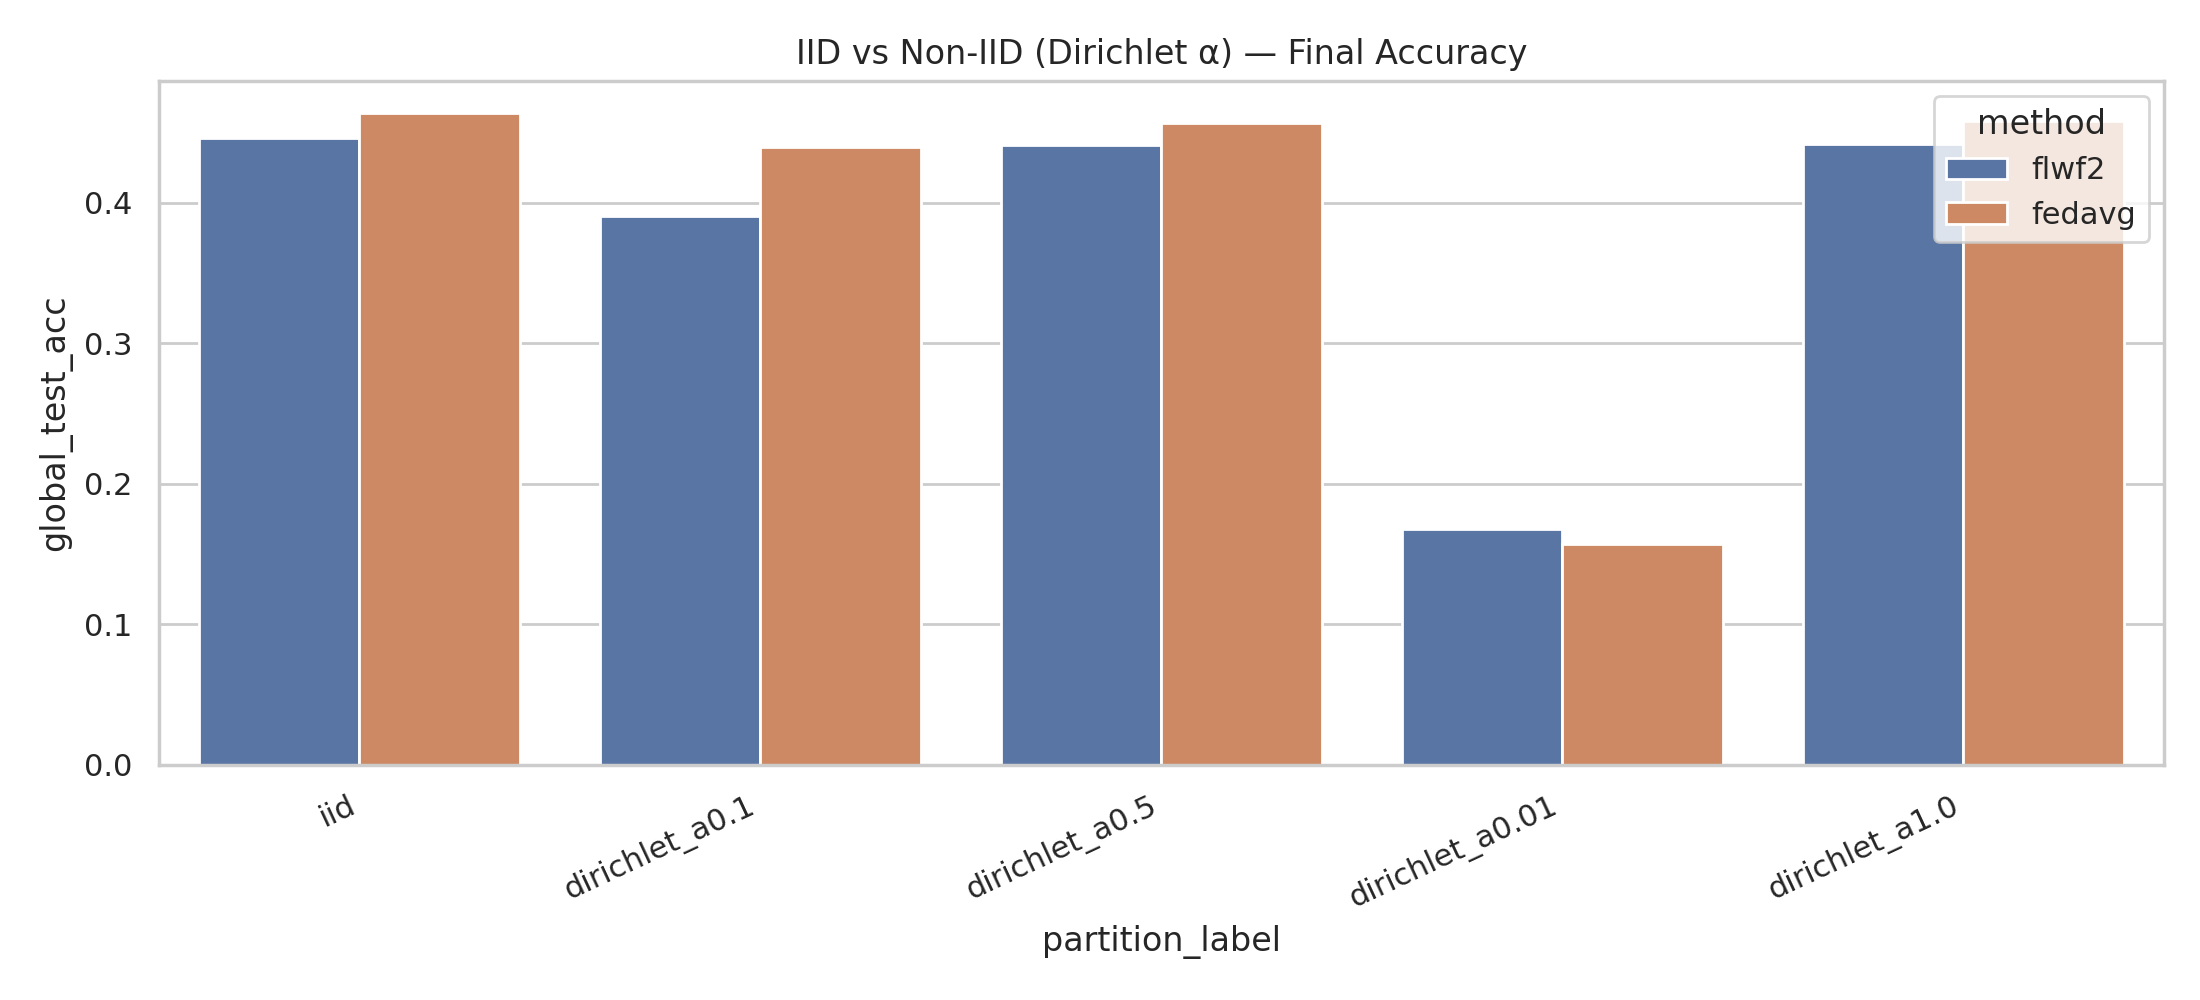
\includegraphics[width=\columnwidth]{images/iid_vs_noniid_final_accuracy.png}
\caption{Final-round global test accuracy for FedAvg and FLwF-2 under
all five partition regimes (IID and $\mathrm{Dir}(\alpha)$,
$\alpha\in\{0.01,0.1,0.5,1.0\}$), aggregated across all
(dataset, $K$) combinations. Bars are means; error bars are dropped
for clarity. Source: \texttt{src/analyze.py}.}
\label{fig:iid_vs_noniid}
\end{figure}

\subsection{Convergence and Forgetting over Rounds}

Figures~\ref{fig:acc_rounds}--\ref{fig:forgetting_rounds} plot global
accuracy, loss and the Task~1 forgetting metric versus round. All
three show the same picture: both methods climb to a Task-1 plateau
($\approx 49\%$ on MNIST/FMNIST, the upper bound when only Task~1
classes are testable) in the first ten rounds; at round 11 the task
switches and FedAvg's forgetting jumps to $\sim\!1$ within a few
rounds, whereas FLwF-2 keeps it pinned near zero for the rest of the
run. Figure~\ref{fig:method_box} confirms this as a per-method
distribution: FLwF-2's stability prior bounds its variance, while
FedAvg occasionally collapses below $20\%$ in the most extreme
non-IID configurations.

\begin{figure}[t]
\centering
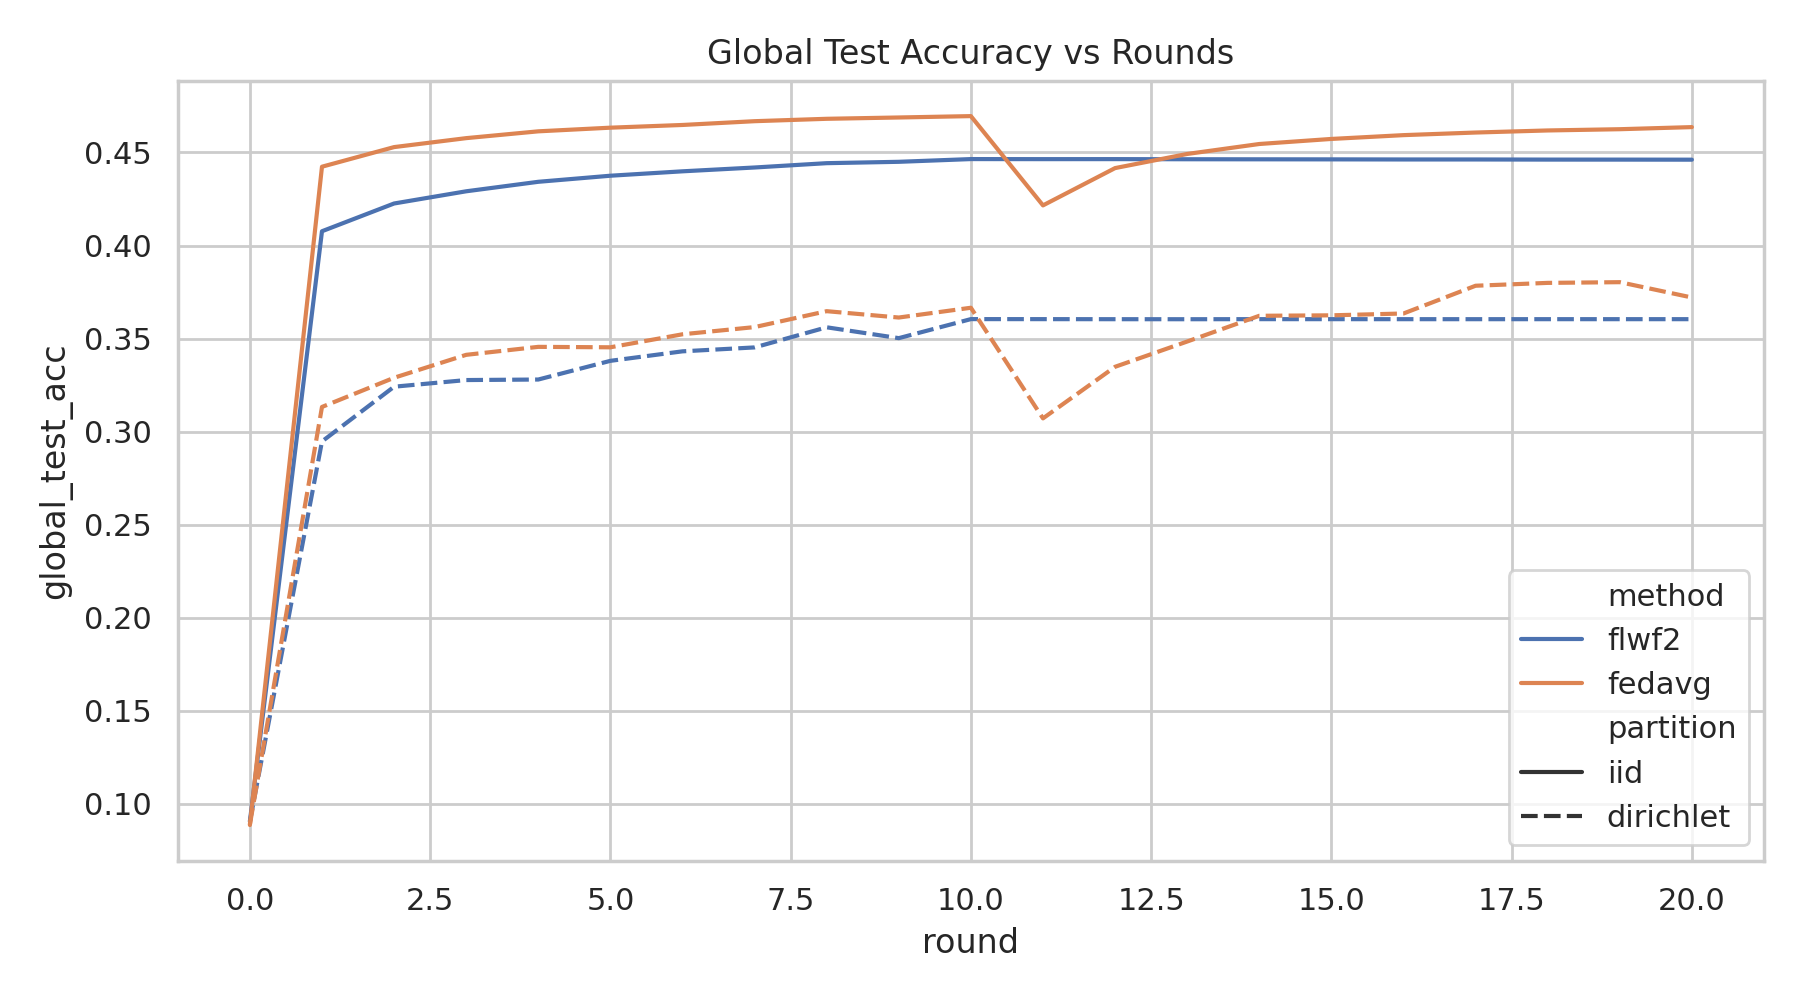
\includegraphics[width=\columnwidth]{images/accuracy_vs_rounds.png}
\caption{Global test accuracy versus communication rounds across all
runs (lines coloured by method, styled by partition). The drop at
round 11 is the Task~1 $\to$ Task~2 boundary.}
\label{fig:acc_rounds}
\end{figure}

\begin{figure}[t]
\centering
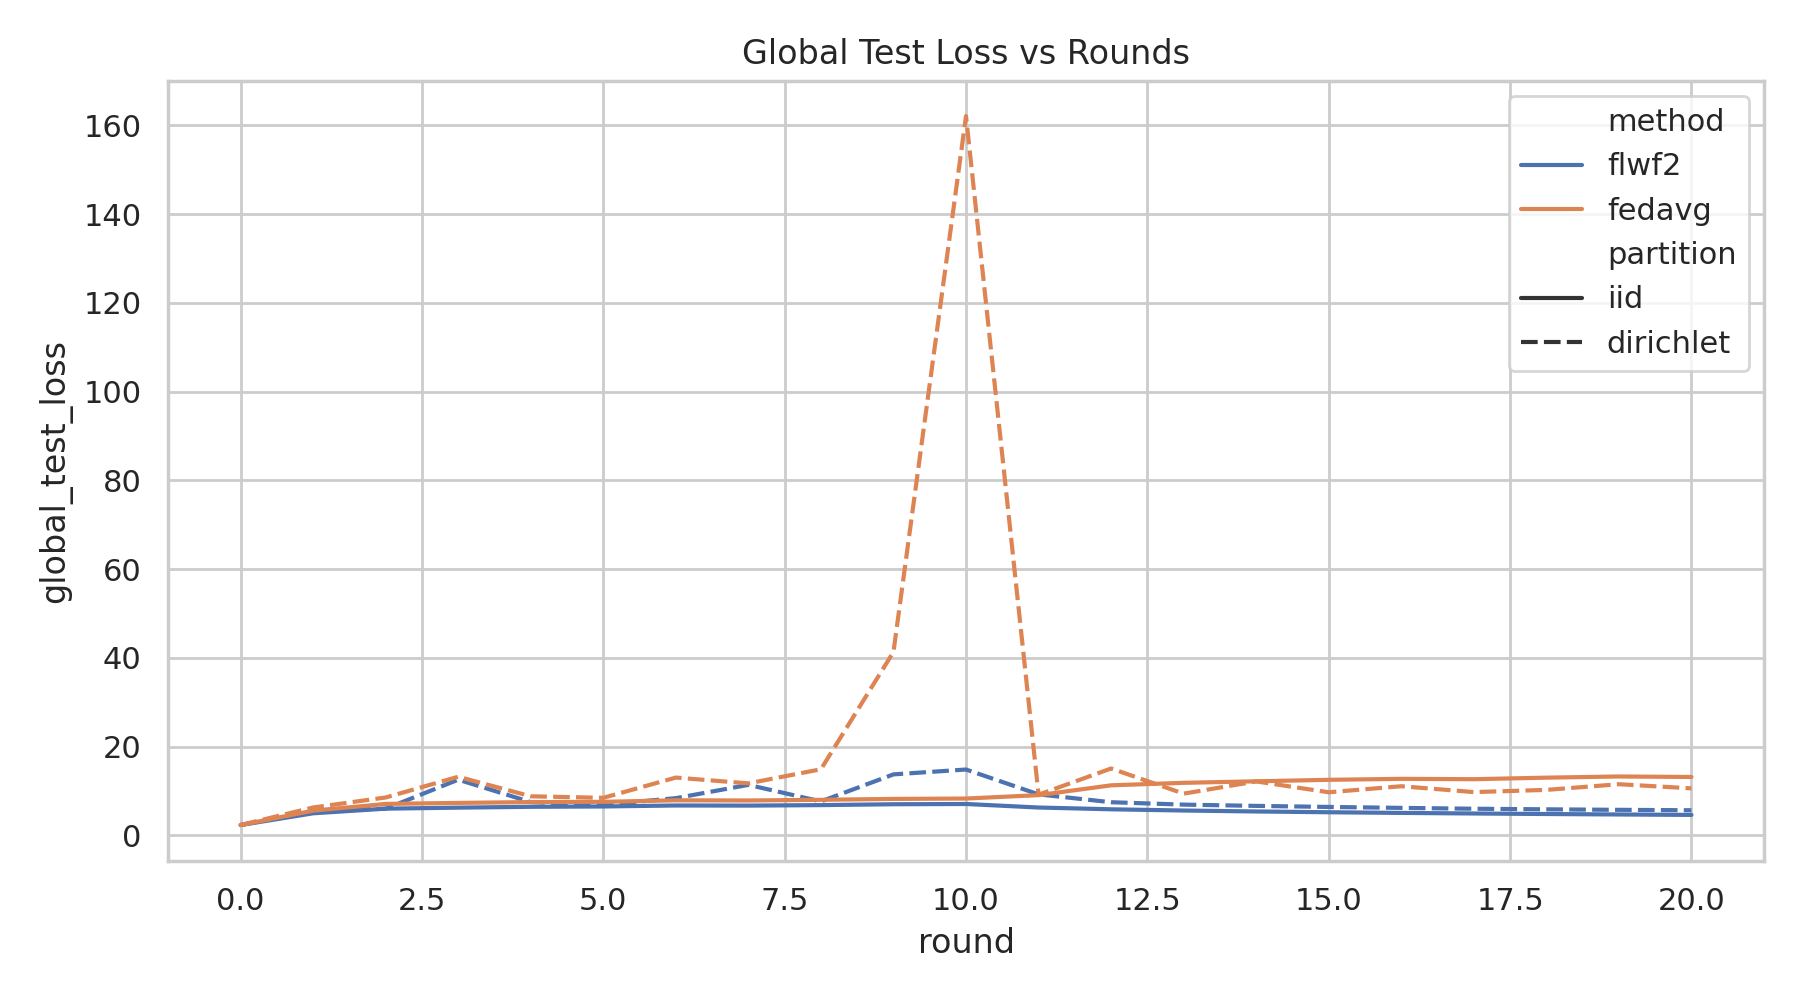
\includegraphics[width=\columnwidth]{images/loss_vs_rounds.png}
\caption{Global test loss versus rounds across all runs.}
\label{fig:loss_rounds}
\end{figure}

\begin{figure}[t]
\centering
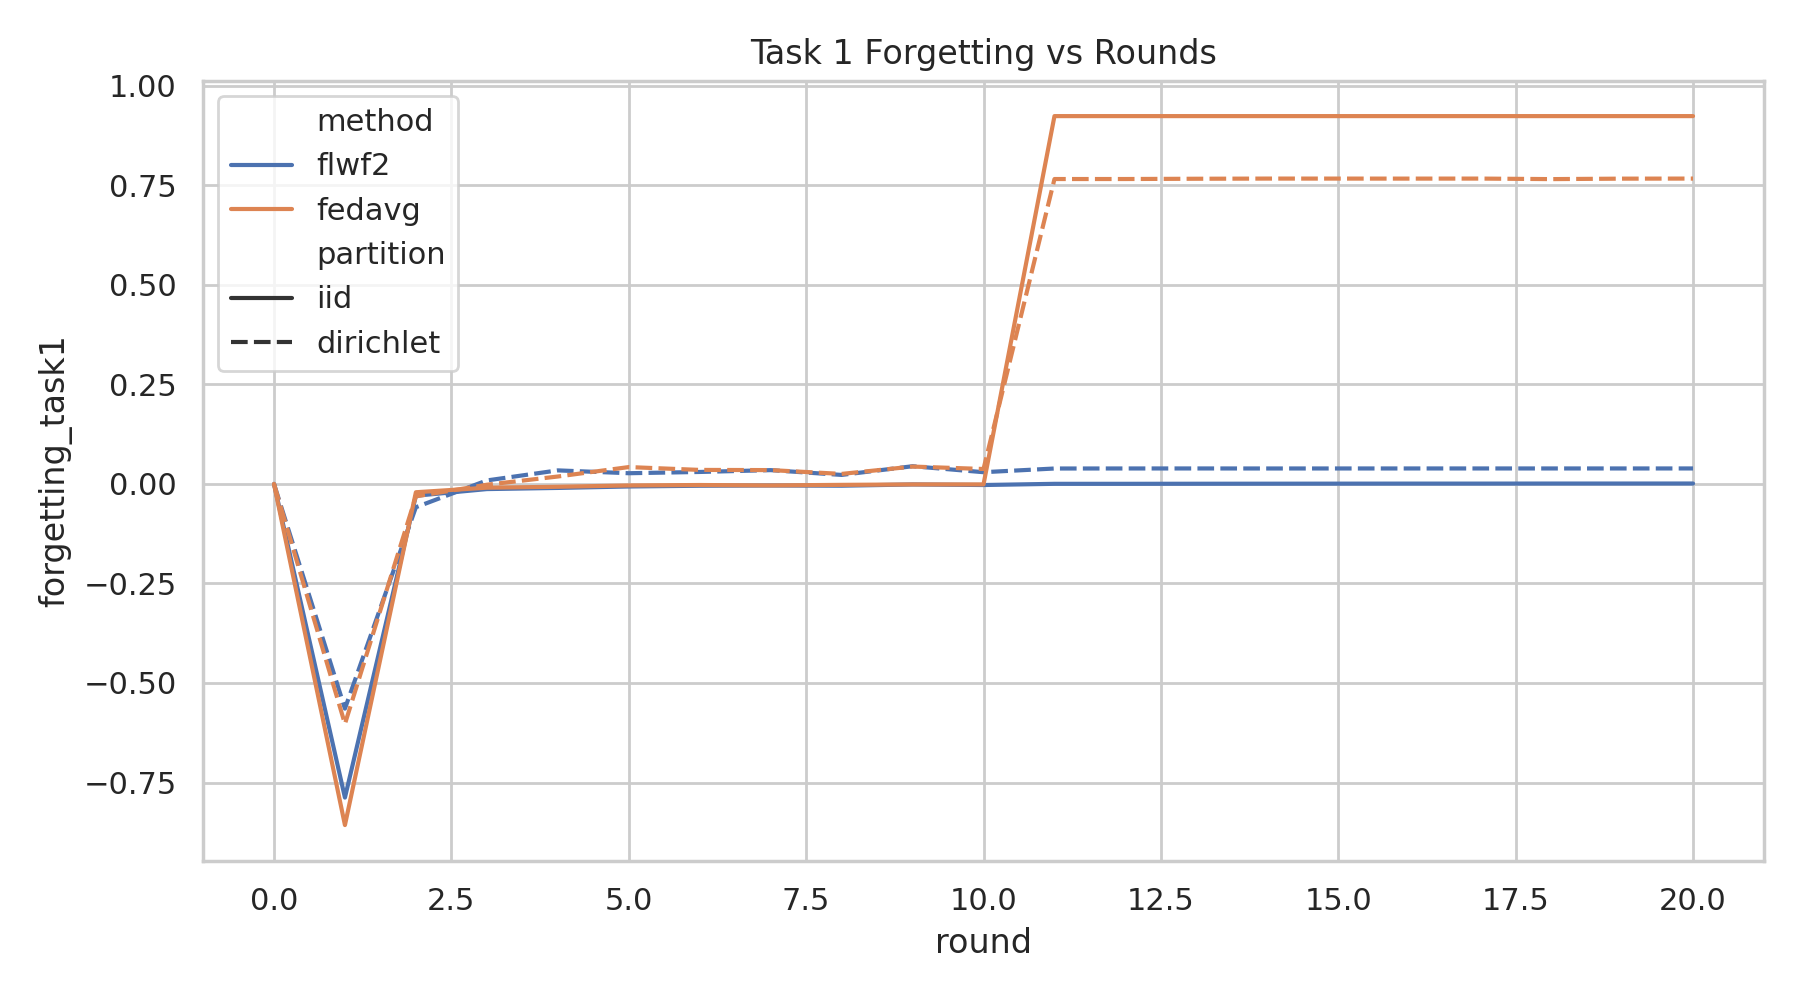
\includegraphics[width=\columnwidth]{images/forgetting_vs_rounds.png}
\caption{Catastrophic-forgetting metric for Task~1 versus round.
FedAvg climbs to $\approx 1$ shortly after the task switch; FLwF-2
keeps it near $0$.}
\label{fig:forgetting_rounds}
\end{figure}

\begin{figure}[t]
\centering
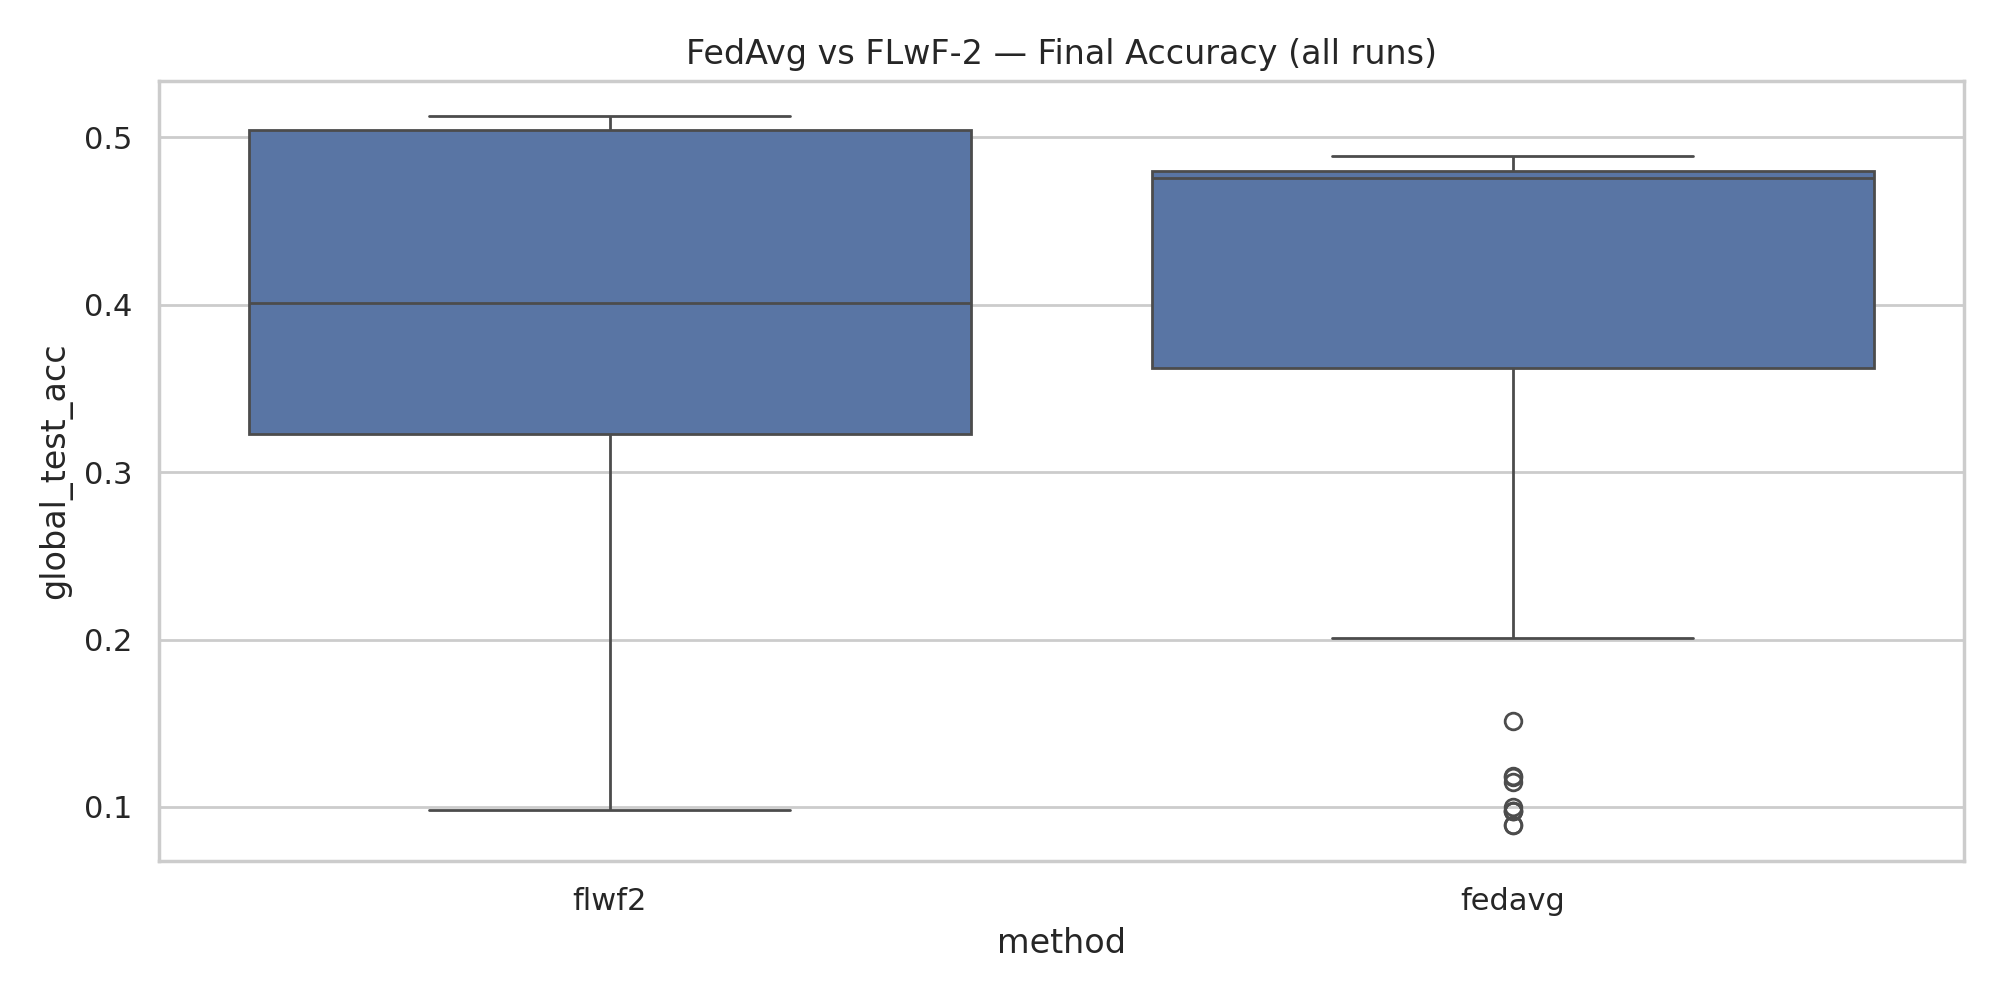
\includegraphics[width=\columnwidth]{images/fedavg_vs_flwf2_final_accuracy.png}
\caption{Distribution of final-round global accuracy across the full
sweep, per method.}
\label{fig:method_box}
\end{figure}

\subsection{Communication Cost}

Both methods exchange the same FP32 weights, so cumulative
communication cost depends only on model size, $K$, and number of
rounds. With our 60{,}654-parameter CNN ($\approx 241.4$~KB/message),
20 rounds and $\rho{=}0.5$, totals are $47.8$, $239.1$ and
$478.3$~MB for $K{=}10,50,100$ respectively (full per-run values in
Table~\ref{tab:full_results}). FLwF-2 derives both teachers locally
and therefore adds no communication overhead.

%==================================================================
\section{Analysis}
\label{sec:analysis}
%==================================================================

\subsection{The Stability--Plasticity Tradeoff}

Equation~\ref{eq:flwf2-loss} weights cross-entropy by $\alpha_{CE}{=}0.001$
and the prior-knowledge KD term by $\beta_{KD}{=}0.7$. The new-task
gradient signal carries effective weight only $0.001$, while the two
teachers --- both unaware of Task~2 --- jointly carry weight $0.999$.
With this configuration, FLwF-2 has essentially no incentive to deviate
from the previous model on Task-2 batches, which is exactly what we
observe: Task~2 accuracy stays near $0\%$ throughout rounds 11--20.
This is not an implementation bug; it is the predicted equilibrium of
the loss with these hyperparameters and a class-incremental split.
The original paper anticipated this and proposed a
\emph{FLwF-2 + Fine-Tuning} hybrid that switches the loss weighting
adaptively. We deliberately stayed with the literal hyperparameters to
isolate the dual-teacher contribution.

\subsection{Effect of Client Count}

Across all three datasets, increasing $K$ from 10 to 100 (with
$\rho{=}0.5$ fixed, so the number of sampled clients per round grows
linearly) produces a small accuracy drop, primarily because each
client's local dataset shrinks and per-client gradient noise
increases. The effect is mild on MNIST and FMNIST (well within
$\pm 2\%$ for both methods at IID) and more pronounced on CIFAR-10
($\approx 5{-}6\%$ between $K{=}10$ and $K{=}100$).

\subsection{Effect of Dirichlet $\alpha$}

For $\alpha\!\in\!\{0.5,1.0\}$ and IID, both methods reach near-clean
Task accuracy. At $\alpha\!=\!0.1$ both still converge but to a lower
plateau. At $\alpha\!=\!0.01$, label distribution is essentially
single-class per client; both methods collapse to $\approx 10\%$ on
MNIST/CIFAR-10 and roughly fail to separate the classes. FLwF-2
inherits this failure mode --- the dual-teacher prior cannot rescue an
underlying federation that has no consistent gradient signal.

\subsection{Backward Transfer and Convergence Round}

Because FLwF-2 freezes most of the prior representation, its backward
transfer on Task~1 is essentially zero ($\le 0.5\%$ change after
Task~2), whereas FedAvg's BWT is strongly negative ($\approx -1.0$ on
MNIST), as expected.

The course-mandated convergence-round metric (smallest round at which
\emph{global} accuracy first reaches $80\%$) is undefined in our
class-incremental setting: only one half of the label space is
testable at a time, so the global ceiling is $\approx 50\%$ by
construction and no run attains $80\%$. We therefore report ``n/a''
in Table~\ref{tab:full_results} rather than fabricate a value;
redefining the metric per active task is left to future work.

%==================================================================
\section{Limitations and Future Work}
\label{sec:limitations}
%==================================================================

\paragraph{Limitations.}
We use only two tasks, the literal $(\alpha_{CE},\beta_{KD})$ from
the original paper, and a homogeneous CNN. We do not compare against
FLwF-1 or the FLwF-2 + Fine-Tuning hybrid.

\paragraph{Future Work.}
The most direct next step is an adaptive
$(\alpha_{CE},\beta_{KD})$ schedule that interpolates between the
plasticity and stability extremes (e.g.\ start plastic, anneal
towards stability), or equivalently the FLwF-2 + Fine-Tuning hybrid
proposed in~\cite{flwf}. Beyond that: longer task sequences on
CIFAR-100, soft-label-only exchange à la FedMD~\cite{fedmd}~/
FedDF~\cite{feddf} for architecture-heterogeneous federations, and
a privacy analysis quantifying any incremental leakage from sharing
weights versus soft labels.

%==================================================================
\section{Conclusion}
\label{sec:conclusion}
%==================================================================

A 90-run sweep of FedAvg and FLwF-2 in Flower~+~PyTorch confirms that
dual-teacher distillation eliminates catastrophic forgetting at zero
extra communication cost, but with the literal
$(\alpha_{CE},\beta_{KD})=(0.001,0.7)$ it does so at the cost of
near-zero plasticity --- the mirror image of FedAvg's high-plasticity,
high-forgetting failure mode. The natural next step is an adaptive
scheme that interpolates between these extremes; our resume-safe
sweep harness is designed to make such follow-up experiments
straightforward.

%==================================================================
\appendix
\section{Full Results Table}
\label{app:results}
%==================================================================

Table~\ref{tab:full_results} reports the complete per-configuration
summary. ``Acc'' is final-round global test accuracy ($\%$),
``Comm.'' is cumulative communication cost in MB (full-weight, both
directions, FP32) and ``Forgetting'' is for Task~1. Convergence-round
is omitted for the reason given in Section~\ref{sec:analysis}.

% Full per-configuration results table (Appendix).
\begin{table*}[t]
\centering
\caption{Full experimental results summary across all 90 configurations.}
\label{tab:full_results}
\renewcommand{\arraystretch}{1.1}
\small
\begin{tabular}{llcccccc}
\toprule
\textbf{Method} & \textbf{Dataset} & \textbf{$K$}
 & \textbf{Partition} & \textbf{Rounds}
 & \textbf{Acc (\%)} & \textbf{Comm.\ (MB)} & \textbf{Forgetting} \\
\midrule
FedAvg & MNIST    &  10 & IID       & 20 &  48.3 &   47.8 & 1.00 \\
FedAvg & MNIST    &  10 & Dir(0.01) & 20 &  10.0 &   47.8 & 0.41 \\
FedAvg & MNIST    &  10 & Dir(0.1)  & 20 &  47.6 &   47.8 & 0.99 \\
FedAvg & MNIST    &  10 & Dir(0.5)  & 20 &  48.2 &   47.8 & 1.00 \\
FedAvg & MNIST    &  10 & Dir(1.0)  & 20 &  48.3 &   47.8 & 1.00 \\
FedAvg & MNIST    &  50 & IID       & 20 &  48.0 &  239.1 & 0.99 \\
FedAvg & MNIST    &  50 & Dir(0.01) & 20 &   9.7 &  239.1 & 0.24 \\
FedAvg & MNIST    &  50 & Dir(0.1)  & 20 &  44.8 &  239.1 & 0.97 \\
FedAvg & MNIST    &  50 & Dir(0.5)  & 20 &  47.9 &  239.1 & 0.99 \\
FedAvg & MNIST    &  50 & Dir(1.0)  & 20 &  47.9 &  239.1 & 0.99 \\
FedAvg & MNIST    & 100 & IID       & 20 &  47.8 &  478.3 & 0.99 \\
FedAvg & MNIST    & 100 & Dir(0.01) & 20 &  30.9 &  478.3 & 0.54 \\
FedAvg & MNIST    & 100 & Dir(0.1)  & 20 &  46.6 &  478.3 & 0.98 \\
FedAvg & MNIST    & 100 & Dir(0.5)  & 20 &  47.8 &  478.3 & 0.99 \\
FedAvg & MNIST    & 100 & Dir(1.0)  & 20 &  47.6 &  478.3 & 0.99 \\
\midrule
FedAvg & FMNIST   &  10 & IID       & 20 &  48.9 &   47.8 & 0.94 \\
FedAvg & FMNIST   &  10 & Dir(0.01) & 20 &  20.1 &   47.8 & 0.60 \\
FedAvg & FMNIST   &  10 & Dir(0.1)  & 20 &  47.6 &   47.8 & 0.83 \\
FedAvg & FMNIST   &  10 & Dir(0.5)  & 20 &  48.6 &   47.8 & 0.93 \\
FedAvg & FMNIST   &  10 & Dir(1.0)  & 20 &  48.7 &   47.8 & 0.93 \\
FedAvg & FMNIST   &  50 & IID       & 20 &  48.5 &  239.1 & 0.91 \\
FedAvg & FMNIST   &  50 & Dir(0.01) & 20 &  30.5 &  239.1 & 0.51 \\
FedAvg & FMNIST   &  50 & Dir(0.1)  & 20 &  47.9 &  239.1 & 0.81 \\
FedAvg & FMNIST   &  50 & Dir(0.5)  & 20 &  48.2 &  239.1 & 0.91 \\
FedAvg & FMNIST   &  50 & Dir(1.0)  & 20 &  48.3 &  239.1 & 0.91 \\
FedAvg & FMNIST   & 100 & IID       & 20 &  48.0 &  478.3 & 0.90 \\
FedAvg & FMNIST   & 100 & Dir(0.01) & 20 &  31.1 &  478.3 & 0.57 \\
FedAvg & FMNIST   & 100 & Dir(0.1)  & 20 &  46.7 &  478.3 & 0.82 \\
FedAvg & FMNIST   & 100 & Dir(0.5)  & 20 &  47.9 &  478.3 & 0.90 \\
FedAvg & FMNIST   & 100 & Dir(1.0)  & 20 &  48.0 &  478.3 & 0.90 \\
\midrule
FedAvg & CIFAR-10 &  10 & IID       & 20 &  43.2 &   48.3 & 0.80 \\
FedAvg & CIFAR-10 &  10 & Dir(0.01) & 20 &  11.5 &   48.3 & 0.45 \\
FedAvg & CIFAR-10 &  10 & Dir(0.1)  & 20 &  36.3 &   48.3 & 0.60 \\
FedAvg & CIFAR-10 &  10 & Dir(0.5)  & 20 &  40.7 &   48.3 & 0.79 \\
FedAvg & CIFAR-10 &  10 & Dir(1.0)  & 20 &  42.3 &   48.3 & 0.78 \\
FedAvg & CIFAR-10 &  50 & IID       & 20 &  38.8 &  241.4 & 0.74 \\
FedAvg & CIFAR-10 &  50 & Dir(0.01) & 20 &  11.8 &  241.4 & 0.32 \\
FedAvg & CIFAR-10 &  50 & Dir(0.1)  & 20 &  36.2 &  241.4 & 0.67 \\
FedAvg & CIFAR-10 &  50 & Dir(0.5)  & 20 &  35.0 &  241.4 & 0.73 \\
FedAvg & CIFAR-10 &  50 & Dir(1.0)  & 20 &  37.7 &  241.4 & 0.72 \\
FedAvg & CIFAR-10 & 100 & IID       & 20 &  37.4 &  482.9 & 0.69 \\
FedAvg & CIFAR-10 & 100 & Dir(0.01) & 20 &  11.9 &  482.9 & 0.30 \\
FedAvg & CIFAR-10 & 100 & Dir(0.1)  & 20 &  33.4 &  482.9 & 0.62 \\
FedAvg & CIFAR-10 & 100 & Dir(0.5)  & 20 &  36.7 &  482.9 & 0.67 \\
FedAvg & CIFAR-10 & 100 & Dir(1.0)  & 20 &  36.7 &  482.9 & 0.67 \\
\midrule
FLwF-2 & MNIST    &  10 & IID       & 20 &  51.3 &   47.8 & \textbf{0.00} \\
FLwF-2 & MNIST    &  10 & Dir(0.01) & 20 &   9.8 &   47.8 & 0.15 \\
FLwF-2 & MNIST    &  10 & Dir(0.1)  & 20 &  50.5 &   47.8 & \textbf{0.01} \\
FLwF-2 & MNIST    &  10 & Dir(0.5)  & 20 &  51.2 &   47.8 & \textbf{0.00} \\
FLwF-2 & MNIST    &  10 & Dir(1.0)  & 20 &  51.2 &   47.8 & \textbf{0.00} \\
FLwF-2 & MNIST    &  50 & IID       & 20 &  51.1 &  239.1 & \textbf{0.00} \\
FLwF-2 & MNIST    &  50 & Dir(0.01) & 20 &   9.8 &  239.1 & 0.20 \\
FLwF-2 & MNIST    &  50 & Dir(0.1)  & 20 &  50.6 &  239.1 & \textbf{0.00} \\
FLwF-2 & MNIST    &  50 & Dir(0.5)  & 20 &  51.0 &  239.1 & \textbf{0.00} \\
FLwF-2 & MNIST    &  50 & Dir(1.0)  & 20 &  51.1 &  239.1 & \textbf{0.00} \\
FLwF-2 & MNIST    & 100 & IID       & 20 &  50.9 &  478.3 & \textbf{0.00} \\
FLwF-2 & MNIST    & 100 & Dir(0.01) & 20 &  30.0 &  478.3 & \textbf{0.00} \\
FLwF-2 & MNIST    & 100 & Dir(0.1)  & 20 &  50.4 &  478.3 & \textbf{0.00} \\
FLwF-2 & MNIST    & 100 & Dir(0.5)  & 20 &  50.8 &  478.3 & \textbf{0.00} \\
FLwF-2 & MNIST    & 100 & Dir(1.0)  & 20 &  50.9 &  478.3 & \textbf{0.00} \\
\midrule
FLwF-2 & FMNIST   &  10 & IID       & 20 &  46.7 &   47.8 & \textbf{0.00} \\
FLwF-2 & FMNIST   &  10 & Dir(0.01) & 20 &  32.3 &   47.8 & \textbf{0.00} \\
FLwF-2 & FMNIST   &  10 & Dir(0.1)  & 20 &  37.0 &   47.8 & 0.09 \\
FLwF-2 & FMNIST   &  10 & Dir(0.5)  & 20 &  46.5 &   47.8 & \textbf{0.00} \\
FLwF-2 & FMNIST   &  10 & Dir(1.0)  & 20 &  46.1 &   47.8 & \textbf{0.01} \\
FLwF-2 & FMNIST   &  50 & IID       & 20 &  45.7 &  239.1 & \textbf{0.00} \\
FLwF-2 & FMNIST   &  50 & Dir(0.01) & 20 &  11.2 &  239.1 & 0.15 \\
FLwF-2 & FMNIST   &  50 & Dir(0.1)  & 20 &  40.8 &  239.1 & \textbf{0.00} \\
FLwF-2 & FMNIST   &  50 & Dir(0.5)  & 20 &  45.3 &  239.1 & \textbf{0.00} \\
FLwF-2 & FMNIST   &  50 & Dir(1.0)  & 20 &  45.5 &  239.1 & \textbf{0.00} \\
FLwF-2 & FMNIST   & 100 & IID       & 20 &  44.9 &  478.3 & \textbf{0.00} \\
FLwF-2 & FMNIST   & 100 & Dir(0.01) & 20 &  27.0 &  478.3 & \textbf{0.00} \\
FLwF-2 & FMNIST   & 100 & Dir(0.1)  & 20 &  34.5 &  478.3 & 0.13 \\
FLwF-2 & FMNIST   & 100 & Dir(0.5)  & 20 &  45.2 &  478.3 & \textbf{0.00} \\
FLwF-2 & FMNIST   & 100 & Dir(1.0)  & 20 &  44.9 &  478.3 & \textbf{0.00} \\
\midrule
FLwF-2 & CIFAR-10 &  10 & IID       & 20 &  40.1 &   48.3 & \textbf{0.00} \\
FLwF-2 & CIFAR-10 &  10 & Dir(0.01) & 20 &  10.0 &   48.3 & 0.26 \\
FLwF-2 & CIFAR-10 &  10 & Dir(0.1)  & 20 &  27.2 &   48.3 & 0.06 \\
FLwF-2 & CIFAR-10 &  10 & Dir(0.5)  & 20 &  39.3 &   48.3 & \textbf{0.00} \\
FLwF-2 & CIFAR-10 &  10 & Dir(1.0)  & 20 &  38.3 &   48.3 & \textbf{0.01} \\
FLwF-2 & CIFAR-10 &  50 & IID       & 20 &  36.7 &  241.4 & \textbf{0.00} \\
FLwF-2 & CIFAR-10 &  50 & Dir(0.01) & 20 &  11.1 &  241.4 & 0.07 \\
FLwF-2 & CIFAR-10 &  50 & Dir(0.1)  & 20 &  28.9 &  241.4 & 0.09 \\
FLwF-2 & CIFAR-10 &  50 & Dir(0.5)  & 20 &  34.4 &  241.4 & \textbf{0.04} \\
FLwF-2 & CIFAR-10 &  50 & Dir(1.0)  & 20 &  36.0 &  241.4 & \textbf{0.00} \\
FLwF-2 & CIFAR-10 & 100 & IID       & 20 &  34.1 &  482.9 & \textbf{0.00} \\
FLwF-2 & CIFAR-10 & 100 & Dir(0.01) & 20 &   9.9 &  482.9 & 0.10 \\
FLwF-2 & CIFAR-10 & 100 & Dir(0.1)  & 20 &  31.8 &  482.9 & \textbf{0.00} \\
FLwF-2 & CIFAR-10 & 100 & Dir(0.5)  & 20 &  33.0 &  482.9 & \textbf{0.00} \\
FLwF-2 & CIFAR-10 & 100 & Dir(1.0)  & 20 &  33.6 &  482.9 & \textbf{0.00} \\
\bottomrule
\end{tabular}
\end{table*}


%==================================================================
\bibliographystyle{IEEEtran}
\begin{thebibliography}{99}

\bibitem{fedavg}
B. McMahan, E. Moore, D. Ramage, S. Hampson, and B. A. y Arcas,
``Communication-efficient learning of deep networks from decentralized data,''
\textit{Proc. Artif. Intell. Statist.}, pp.\ 1273--1282, 2017.

\bibitem{flwf}
A. Usmanova, F. Portet, P. Lalanda, and G. Vega,
``Federated continual learning through distillation in pervasive computing,''
\textit{arXiv:2207.08181}, 2022.

\bibitem{hinton_kd}
G. Hinton, O. Vinyals, and J. Dean,
``Distilling the knowledge in a neural network,''
\textit{NIPS Deep Learning Workshop}, 2015.

\bibitem{forgetting}
J. Kirkpatrick et al.,
``Overcoming catastrophic forgetting in neural networks,''
\textit{Proc. Natl. Acad. Sci.}, vol.\ 114, no.\ 13, pp.\ 3521--3526, 2017.

\bibitem{flower}
D. J. Beutel et al.,
``Flower: A friendly federated learning research framework,''
\textit{arXiv:2007.14390}, 2020.

\bibitem{lwf}
Z. Li and D. Hoiem,
``Learning without forgetting,''
\textit{IEEE Trans. Pattern Anal. Mach. Intell.}, vol.\ 40, pp.\ 2935--2947, 2017.

\bibitem{feddf}
T. Lin, L. Kong, S. U. Stich, and M. Jaggi,
``Ensemble distillation for robust model fusion in federated learning,''
\textit{Proc. NeurIPS}, vol.\ 33, pp.\ 2351--2363, 2020.

\bibitem{fedmd}
D. Li and J. Wang,
``FedMD: Heterogenous federated learning via model distillation,''
\textit{NeurIPS Workshop}, 2019.

\bibitem{fedprox}
T. Li, A. K. Sahu, M. Zaheer, M. Sanjabi, A. Talwalkar, and V. Smith,
``Federated optimization in heterogeneous networks,''
\textit{Proc. MLSys}, vol.\ 2, pp.\ 429--450, 2020.

\bibitem{dirichlet}
K.-W. Ng, G.-L. Tian, and M.-L. Tang,
``Dirichlet and related distributions: Theory, methods and applications,''
Wiley Series in Probability and Statistics, Wiley, 2011.

\end{thebibliography}

\end{document}
